\documentclass[a4paper,11pt,oneside]{article}

\usepackage{amsmath,amssymb,epsfig}
\usepackage[T1]{fontenc}
\usepackage{ae,aecompl}
\usepackage{url}
\usepackage{subfigure}
\addtolength{\voffset}{-1cm}
\addtolength{\hoffset}{-1cm}
\setlength{\parindent}{0in}
\addtolength{\textwidth}{1.8cm}
\addtolength{\textheight}{1cm}
\addtolength{\parskip}{.5cm}

% Example definitions.
% --------------------
\def\e{{e^{j\omega}}}
\def\W{{W_M}}
\def\sumk{{\sum_{k=-\infty}^{\infty}}}
\def\x{{\mathbf x}}
\def\X{{\mathbf X}}
\def\Y{{\mathbf Y}}
\def\u{{\mathbf u}}
\def\U{{\mathbf U}}
\def\x{{\mathbf x}}
\def\s{{\mathbf s}}
\def\A{{\mathbf A}}
\def\y{{\mathbf y}}
\def\w{{\mathbf w}}
\def\B{{\mathbf B}}
\def\a{{\mathbf a}}
\def\D{{\mathbf D}}
\def\P{{\mathbf P}}
\def\n{{\mathbf n}}
\def\V{{\mathbf V}}
\def\R{{\mathbf R}}
\def\I{{\mathbf I}}
\def\M{{\mathbf M}}
\def\sech{{\mathrm{sech}}}
\def\L{{\cal L}}
\def\Cum{{\rm{Cum}}}
\def\var{{\rm{var}}}
\def\T{{\mathbf T}}
\def\C{{\mathbf C}}
\def\tf{{\emph{t-f}}}


% Title.
% ------
\title{\large{\textbf{HOMEWORK 4 - SOLUTIONS}}}
\author{SGN-1156 Signal Processing Techniques\\
\url{http://www.cs.tut.fi/courses/SGN-1156}\\
Tampere University of Technology\\
Germ\'an G\'omez-Herrero, \url{http://germangh.com}}
\date{Due: December 2, 2009, 10:00 AM}

\begin{document}
\maketitle

\textbf{QUESTION 1 (7 points):} Compute the 4-point DFTs of the two real sequences:

\begin{itemize}
\item[] $x_{1}=\{1,\;4,\; -2,\; 0\}$
\item[] $x_{2}=\{-2,\; 0,\; 1,\; 3\}$
\end{itemize}

using ONLY a single 4-point DFT.

\vspace{1cm}

\textbf{SOLUTION:}

Since both $x_1[n]$ and $x_2[n]$ are real sequences of the same length their DFTs can be obtained by computing the single DFT of the complex sequence $y[n]=x_1[n]+jx_2[n]$. So, first we define such sequence:

\[
y[n] = x_1[n]+jx_2[n]=\left\{1-2j,4,-2+j,3j\right\}
\]

Then we compute its 4-point DFT using the classical DFT formula or its matrix version. If the length of the DFT is 2 or 4 the matrix form is specially suitable because the entries of the DFT matrix are just real numbers and purely imaginary numbers. By using boldface lowercase letters to denote column vector and boldface uppercase letters to denote matrices, we can write:

\[
\Y = \D_4\y = \left[
\begin{array}{rrrr}
1 & 1 &1 &1\\
1 & -j & -1 & j\\
1 & -1 & 1 & -1\\
1 & j & -1 & j\\
\end{array}
\right]
\cdot
\left[
\begin{array}{r}
1-2j\\
4\\
-2+j\\
3j\\
\end{array}
\right]=
\left[
\begin{array}{r}
3+2j\\
-7j\\
-5-4j\\
6+j
\end{array}
\right]
\]

So we obtained that the DFT of $y[n]$ is $Y[k]=\left\{3+2j,\;-7j,\;-5-4j,\;6+j\right\}$. Then, the DFT of $x_1[n]$ and $x_2[n]$ are given by:

\begin{equation}\label{eq1}
\begin{array}{lll}
X_1[k] &=& \frac{1}{2}\left[Y[k]+Y^*[<-k>_{4}]\right]\\
X_2[k] &=& \frac{1}{2j}\left[Y[k]-Y^*[<-k>_{4}]\right]\\
\end{array}
\end{equation}

In the two equations above we have the term $Y^*[<-k>_{4}]$ which is the complex conjugate of the circularly time-reversed version of $Y[k]$. The easiest way of obtaining $Y[<-k>_{4}]$ is graphically:

\begin{figure}[h!]
\centering
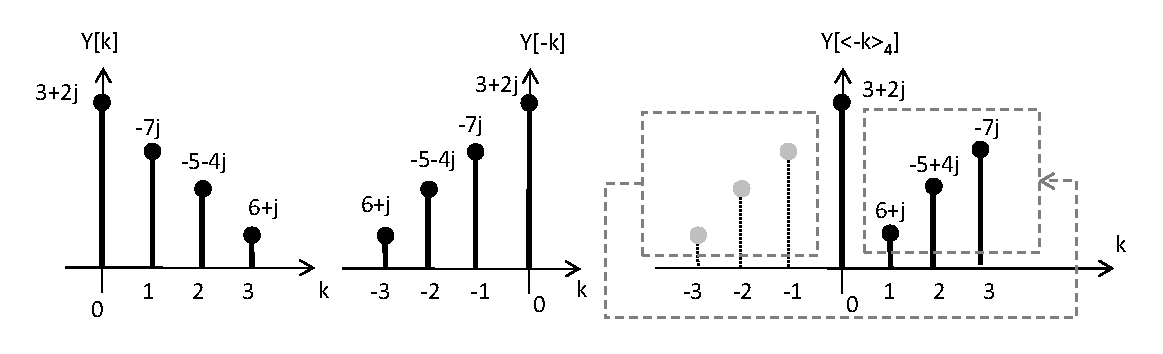
\includegraphics[width=\textwidth]{fig1.eps}
\caption{Circular time-reversal of sequence $Y[k]$. Note that the length of the lines representing each point of the sequence are arbitrary (unrelated to the actual complex value of those points) and should be understood just a means of differentiating between the different points of the sequence.}
\label{fig1}
\end{figure} 

So we obtained that $Y[<-k>_{4}]=\left\{3+2j,\;6+j,\;-5+4j,\;-7j\right\}$ and, therefore, $Y^*[<-k>_{4}]=\left\{3-2j,6-j,-5-4j,+7j\right\}$. Replacing the value of $Y^*[<-k>_{4}]$ in Eq.~\ref{eq1} we finally obtain that:

\[
\begin{array}{lllll}
X_1[k] &=& \frac{1}{2}\left[Y[k]+Y^*[<-k>_{4}]\right]&=&\left\{3,\;3-4j,\;-5,\;3+4j\right\}\\
X_2[k] &=& \frac{1}{2j}\left[Y[k]-Y^*[<-k>_{4}]\right]&=&\left\{2,\; -3+3j,\;-4,\;-3-3j\right\}\\
\end{array}
\]

You can check that what you did above is correct with MATLAB. To replicate the steps above in MATLAB you have to execute these commands:
\begin{verbatim}
x1=[1 4 -2 0];
x2=[-2 0 1 3];
y = x1+j*x2;
Y = fft(y);
Y2 = conj([Y(1) fliplr(Y(2:end))]); % circ. time-revers. + conjug.
X1 = .5*[Y+Y2];
X2 = -.5*j*[Y-Y2];
\end{verbatim}

Alternatively you can compute the DFT of $x_1$ and $x_2$ separately to double-check everything:

\begin{verbatim}
X1fft = fft(x1);
X2fft = fft(x2);
\end{verbatim}

And you can observe that \verb|X1| and \verb|X2|  are identical to \verb|X1fft| and  \verb|X2fft|, respectively.

\vspace{2cm}

\textbf{QUESTION 2 (8 points):} Compute the linear convolution of the two sequences:

\begin{itemize}
\item[] $x_{1}=\{1,\; 1,\; 2,\; -1,\; 0,\; 1\}$
\item[] $x_{2}=\{1,\;-2,\; 3,\; 2,\; 1,\; 0\}$
\end{itemize}

\noindent using the formula of the convolution and using the DFT. Check that both methods yield the same result. For the computations using the DFT you can use MATLAB but giving the exact commands that you typed and explaining why. See the help of functions \verb|fft| and \verb|ifft|.

\vspace{1cm}

\textbf{SOLUTION:}

The linear convolution formula is:

\begin{equation} \label{eq2}
y[n] = \sum_{m=-\infty}^{\infty}x_1[m]x_2[-m+n]
\end{equation}

because the length of $x_1$ is $L_1=6$ and the length of $x_2$ is $L_2=5$, the length of their linear convolution $y[n]$ must be $L_1+L_2-1=10$. So using Eq.~\ref{eq2} for $n=1,...,10$ we obtain that:

\[
y=\{1,\;-1,\;     3,\;     0,\;    11,\;     3,\;    -2,\;     2,\;     2,\;     1\}
\]

this result can be checked using MATLAB:

\begin{verbatim}
x1=[1 1 2 -1 0 1];
x2=[1 -2 3 2 1];
y = conv(x1,x2);
\end{verbatim}

In order to compute the linear convolution of $x_1$ and $x_2$ using the DFT we have to compute the DFT of $L1+L2-1=10$ points of both $x_1$ and $x_2$. This can done in MATLAB with the commands:

\begin{verbatim}
x1=[1 1 2 -1 0 1];
x2=[1 -2 3 2 1];
X1=fft(x1,10);
X2=fft(x2,10);
\end{verbatim}

and then the linear convoltion $y[n]=x_1[n]\otimes x_2[n]$ will just be the inverse DFT of 10 points of the product of the two DFTs that we just computed above:

\begin{verbatim}
y = ifft(X1.*X2,10);
\end{verbatim}

which is equal to the result that we obtained using the formula of the linear convolution.


\vspace{2cm}

\textbf{QUESTION 3 (15 points):} Consider the system shown in Figure~\ref{fig2}. Assume that the input is bandlimited, $X_a(j\Omega)=0$ for $|\Omega|>2\pi\cdot 1000$.

\begin{itemize}
\item[(a)] What constraints must be placed on $L$, $T_1$, and $T_{2}$ in order for $y_a(t)$ to be equal to $x_a(t)$? Sketch the Fourier transforms of $x_a(t)$, $x(n)$, $y(n)$, and $y_a(t)$.
\item[(b)] If $f_1=f_2=20kHz$ and $L=4$, find an expression for $y_a(t)$ in terms of $x_a(t)$. What is the energy of $y_{a}(t)$ with respect to the energy of $x_{a}(t)$?
\end{itemize}

\begin{figure}[h!]
\centering
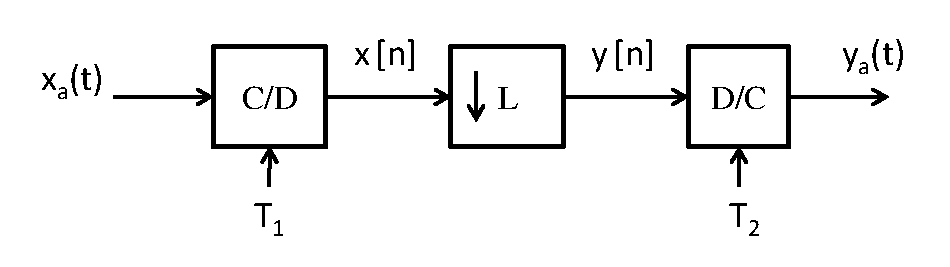
\includegraphics[width=.8\textwidth]{fig2.eps}
\caption{Block diagram of the system of question 3.}
\label{fig2}
\end{figure}



\vspace{1cm}

\textbf{SOLUTION:}

\textbf{(a)}


Without loss of generality, in the following we will assume that the CTFT of the input analog signal $x_a(t)$ looks like depicted in Fig.~\ref{ctftxa}.

\begin{figure}[h!]
\centering
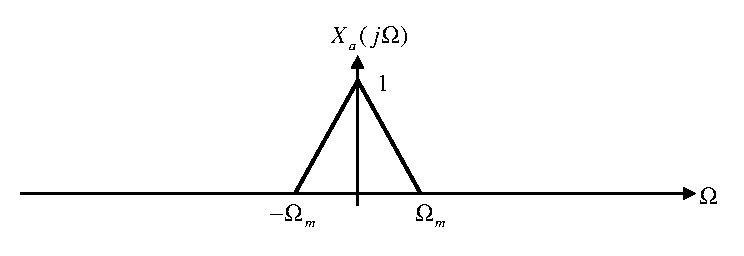
\includegraphics[width=.8\textwidth]{ctftxa.eps}
\caption{CTFT of the input analog signal $x_a(t)$.}
\label{ctftxa}
\end{figure}


where $\Omega_{m}=2\pi\cdot 1000$ is the maximum frequency present in $x_a(t)$. For perfect reconstruction to be possible aliasing in the C/D transformation must be avoided. So the first contraint that has to be fullfiled is:

\begin{equation}\label{const1}
\Omega_1=\frac{2\pi}{T_1}\geq 2\Omega_{m} \Rightarrow T_1\leq  \frac{2\pi}{2\Omega_{m}}=\frac{2\pi}{2\cdot 2\pi\cdot 1000}\Rightarrow T_1\leq 5\cdot 10^{-4} \;\textrm{seconds}
\end{equation}

Remember that in the D/C block take place two subsequent operations. First the input analog signal is multiplied by continuous-time train of impulses having an inter-impulse distance of $T_1$ seconds. The result is also a continuous time signal $x_s(t)$ which is non-zero only in those time instants that are an integer multiple of $T_1$:

\[
x_s(t)=\left\{ 
\begin{array}{lll}
x(t) &\qquad & \textrm{if}\; \frac{t}{T_1}\in\mathbb{Z}\\
0 & \qquad & \textrm{otherwise}
\end{array}
\right.
\]

The CTFT of $x_s(t)$ is depicted in Fig.~\ref{ctftxs}, where $\Delta=\Omega_1-2\Omega_m$ is the spacing between correlative copies of the spectrum of $x_a(t)$. Because we have enforced that $\Omega_1\geq 2\Omega_m$, it is obvious that $\Delta\geq 0$ and therefore there is overlap between two correlative spectral alias, i.e. there is not aliasing.

\begin{figure}[h!]
\centering
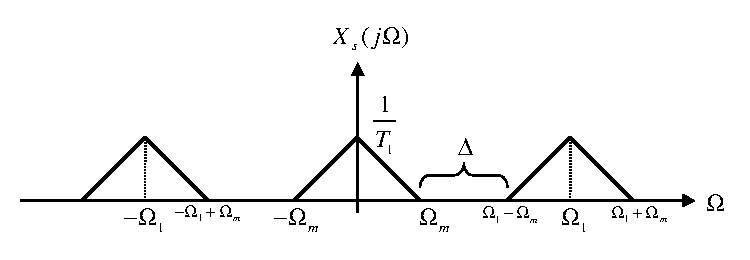
\includegraphics[width=.8\textwidth]{ctftxs.eps}
\caption{CTFT of the continuous-time sampled signal $x_s(t)$.}
\label{ctftxs}
\end{figure}

The DTFT $X(e^{j\omega})$ of the discrete-time signal $x[n]$ has the shape depicted in Fig.~\ref{ctftxs} but with the frequency normalization $\omega=\Omega\cdot T_1=\frac{\Omega\cdot 2\pi}{\Omega_1}$. This DTFT is depicted in Fig.~\ref{dtftx}.

\begin{figure}[h!]
\centering
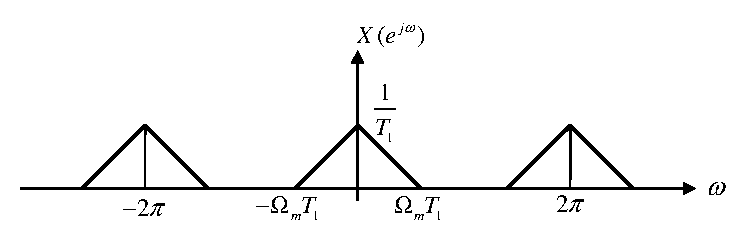
\includegraphics[width=.8\textwidth]{dtftx.eps}
\caption{DTFT of the discrete-time sequence $x[n]$.}
\label{dtftx}
\end{figure}

After the downsampler, the DTFT $Y(e^{j\omega})$ of the sequence $y[n]$ will be the obtained by expanding the frequency range $[-\pi,\pi)$ in Fig.~\ref{dtftx} and replicating the result every $2\pi$. This is depicted in Fig.~\ref{dtfty}.


\begin{figure}[h!]
\centering
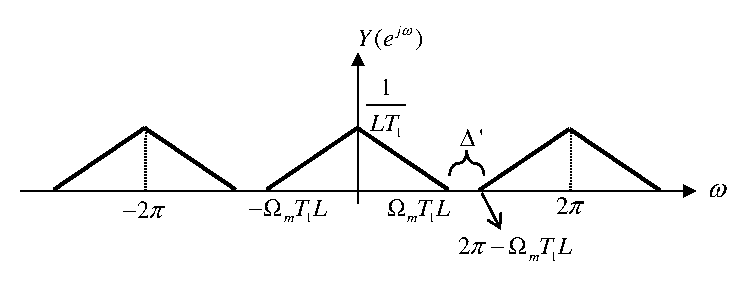
\includegraphics[width=.8\textwidth]{dtfty.eps}
\caption{DTFT of the discrete-time sequence $y[n]$.}
\label{dtfty}
\end{figure}

From Fig.~\ref{dtfty}, it is obvious that for perfect reconstruction to be possible, the space between correlative spectral aliases must be greater than 0, i.e:

\begin{equation}\label{const2}
\Delta'\geq 0 \Rightarrow 2\pi-2\Omega_mT_1L\geq 0 \Rightarrow T_1 \leq \frac{2\pi}{2\Omega_m L} \Rightarrow T_{1} \leq \frac{5\cdot 10^{-4}}{L} \; \textrm{seconds}
\end{equation}

Because $L\geq 2$, the constraint given by Eq.~\ref{const2} is more restrictive that the one found in Eq.~\ref{const1}. Therefore our new constraint for $T_1$ will be the one in Eq.~\ref{const2}.

The D/C block consists of two consecutive operations. First, the input discrete-time sequence $y[n]$ is converted into a continous-time signal $y_s(t)$, which is later passed through an ideal low-pass reconstruction filter with cutoff frequency $\frac{\Omega_m}{2}$ and gain $T_2$ to build the output analog signal $y_a(t)$. The purpose of the reconstruction filter is extract the baseband spectral alias and remove the others. The CTFT $Y_s(j\Omega)$ of $y_s(t)$ is depicted in Fig.~\ref{ctftys}. Clearly, for the reconstruction filter to output a copy of $x_{a}(t)$ the sampling period in the D/C block has to fulfil the constraint: 

\begin{equation}\label{const3}
T_2=T_1\cdot L
\end{equation}

If the condition above is fulfilled then the reconstruction filter will just retain the baseband spectral alias in $Y_s(j\Omega)$ and will amplify it by a factor equal to $T_2=L\cdot T_1$. Thus the CTFT of $y_a(t)$ will be the same as the CTFT of $x_a(t)$, i.e. $y_a(t)=x_a(t)$. So summarizing, the constraints in Eq.~\ref{const2} and Eq.~\ref{const3} have to be fulfilled for perfect reconstruction to occur.

\begin{figure}[h!]
\centering
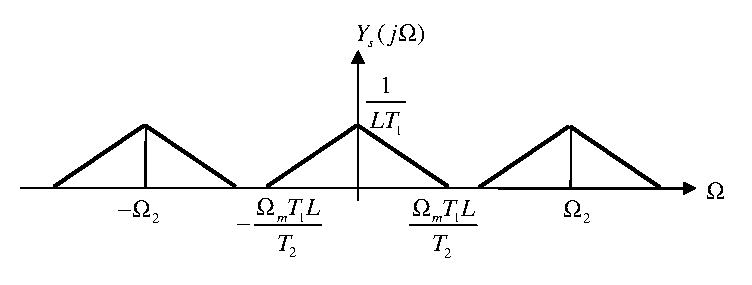
\includegraphics[width=.8\textwidth]{ctftys.eps}
\caption{CTFT of the continous-time signal $y_s(t)$. Notice that this is just the result of de-normalizing the frequencies in Fig.~\ref{dtfty} ($\Omega=\frac{\omega}{T_2}$).}
\label{ctftys}
\end{figure}


\vspace{1cm}
\textbf{(b)}

Since $f_1=f_2=f=2\cdot 10^4$ Hz, the sampling period in both the C/D and D/C blocs will be $T_1=T_2=\frac{1}{f}=5\cdot 10^{-5}$ seconds and their angular sampling frequencies will be $\Omega_s=2\pi f_s=4\cdot 10^{4}\pi$ radians/second. We can see that this sampling period fulfills the constraint in Eq.~\ref{const2}:

\[
T=5\cdot 10^{-5}<\frac{5\cdot 10^{-4}}{L}=\frac{5\cdot 10^{-4}}{4}=12.5\cdot 10^{-5}
\]

Therefore, neither the C/D block nor the downsampler will cause aliasing and the spectral aliases in Fig.~\ref{ctftys} will not overlap each other. In this case, the reconstruction filter will have a cutoff $\frac{\Omega_s}{2}=2\cdot 10^{4}\pi$ radians/seconds so that only the baseband alias in $Y_s(j\Omega)$ is retained. The CTFT of the output analog signal $y_a(t)$ is given in Fig.~\ref{ctfty}.

\begin{figure}[h!]
\centering
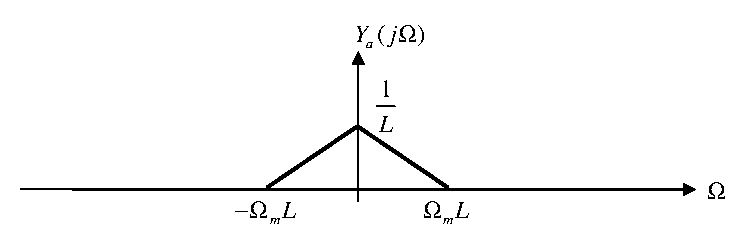
\includegraphics[width=.8\textwidth]{ctfty.eps}
\caption{CTFT of the continous-time output signal $y_a(t)$. Notice that this is just the result of making that $T_1=T_2=T$ in Fig.~\ref{ctftys} and applying a lowpass reconstruction filter with cutoff $\frac{\Omega_s}{2}$ and gain $T$.}
\label{ctfty}
\end{figure}

So we have finally obtained that the relationship between $Y_a(j\Omega)$ and $X_a(j\Omega)$ is:

\begin{equation}\label{relfreq}
Y_a(j\Omega) = \frac{1}{L}X_{a}(\frac{j\Omega}{L})=\frac{1}{4}X_{a}(\frac{j\Omega}{4})
\end{equation}

So the relationship in time domain is:

\begin{equation}
y_a(t)=x_a(Lt)=x_a(4t)
\end{equation}

Then the energy of the output analog signal is (by using Parseval's relation):

\begin{equation}\label{eqenergy}
E_{y_a}=\int_{-\infty}^{\infty}|y_a(t)|^2dt=\frac{1}{2\pi}\int_{-\Omega_mL}^{\Omega_mL}|Y_a(j\Omega)|^2d\Omega
\end{equation}

so using Eq.~\ref{relfreq} we have that:

\begin{equation}\label{energyfreq}
E_{y_a}=\frac{1}{2\pi}\int_{-\Omega_mL}^{\Omega_mL}|\frac{1}{4}X_a(\frac{j\Omega}{4})|^2d\Omega=\frac{1}{16}\cdot\frac{1}{2\pi}\int_{-\Omega_mL}^{\Omega_mL}|X_a(\frac{j\Omega}{4})|^2d\Omega
\end{equation}

and then by making the variable change $\Omega'=\frac{\Omega}{4}$ we have that $d\Omega=4d\Omega'$ and then Eq.~\ref{energyfreq} becomes:

\begin{equation}
E_{y_a}= \frac{4}{16}\cdot\frac{1}{2\pi}\int_{-\Omega_mL}^{\Omega_mL}|X_a(j\Omega')|^2d\Omega'=\frac{1}{4}E_{x_a}
\end{equation}

so the energy of the output signal is one fourth of the energy of the input signal.

The energy of the output could also have been obtained using the time-domain relationship between $y_a(t)$ and $x_a(t)$:

\begin{equation}\label{eqenergytime}
E_{y_a}=\int_{-\infty}^{\infty}|y_a(t)|^2dt=\int_{-\infty}^{\infty}|x_a(4t)|^2dt
\end{equation}

by making the variable change $m=4t$ we have that $dt=\frac{1}{4}dm$ and therefore, Eq.~\ref{eqenergytime} becomes:


\begin{equation}
E_{y_a}=\frac{1}{4}\int_{-\infty}^{\infty}|x_a(m)|^2dm=\frac{1}{4}E_{x_a}
\end{equation}

obtaining the same result that the energy of the ouput is one fourth of the energy of the input.

\end{document}